
%% bare_conf.tex
%% V1.3
%% 2007/01/11
%% by Michael Shell
%% See:
%% http://www.michaelshell.org/
%% for current contact information.
%%
%% This is a skeleton file demonstrating the use of IEEEtran.cls
%% (requires IEEEtran.cls version 1.7 or later) with an IEEE conference paper.
%%
%% Support sites:
%% http://www.michaelshell.org/tex/ieeetran/
%% http://www.ctan.org/tex-archive/macros/latex/contrib/IEEEtran/
%% and
%% http://www.ieee.org/

%%*************************************************************************
%% Legal Notice:
%% This code is offered as-is without any warranty either expressed or
%% implied; without even the implied warranty of MERCHANTABILITY or
%% FITNESS FOR A PARTICULAR PURPOSE! 
%% User assumes all risk.
%% In no event shall IEEE or any contributor to this code be liable for
%% any damages or losses, including, but not limited to, incidental,
%% consequential, or any other damages, resulting from the use or misuse
%% of any information contained here.
%%
%% All comments are the opinions of their respective authors and are not
%% necessarily endorsed by the IEEE.
%%
%% This work is distributed under the LaTeX Project Public License (LPPL)
%% ( http://www.latex-project.org/ ) version 1.3, and may be freely used,
%% distributed and modified. A copy of the LPPL, version 1.3, is included
%% in the base LaTeX documentation of all distributions of LaTeX released
%% 2003/12/01 or later.
%% Retain all contribution notices and credits.
%% ** Modified files should be clearly indicated as such, including  **
%% ** renaming them and changing author support contact information. **
%%
%% File list of work: IEEEtran.cls, IEEEtran_HOWTO.pdf, bare_adv.tex,
%%                    bare_conf.tex, bare_jrnl.tex, bare_jrnl_compsoc.tex
%%*************************************************************************

% *** Authors should verify (and, if needed, correct) their LaTeX system  ***
% *** with the testflow diagnostic prior to trusting their LaTeX platform ***
% *** with production work. IEEE's font choices can trigger bugs that do  ***
% *** not appear when using other class files.                            ***
% The testflow support page is at:
% http://www.michaelshell.org/tex/testflow/



% Note that the a4paper option is mainly intended so that authors in
% countries using A4 can easily print to A4 and see how their papers will
% look in print - the typesetting of the document will not typically be
% affected with changes in paper size (but the bottom and side margins will).
% Use the testflow package mentioned above to verify correct handling of
% both paper sizes by the user's LaTeX system.
%
% Also note that the "draftcls" or "draftclsnofoot", not "draft", option
% should be used if it is desired that the figures are to be displayed in
% draft mode.
%
\documentclass[conference]{IEEEtran}
% Add the compsoc option for Computer Society conferences.
%
% If IEEEtran.cls has not been installed into the LaTeX system files,
% manually specify the path to it like:
% \documentclass[conference]{../sty/IEEEtran}





% Some very useful LaTeX packages include:
% (uncomment the ones you want to load)


% *** MISC UTILITY PACKAGES ***
%
%\usepackage{ifpdf}
% Heiko Oberdiek's ifpdf.sty is very useful if you need conditional
% compilation based on whether the output is pdf or dvi.
% usage:
% \ifpdf
%   % pdf code
% \else
%   % dvi code
% \fi
% The latest version of ifpdf.sty can be obtained from:
% http://www.ctan.org/tex-archive/macros/latex/contrib/oberdiek/
% Also, note that IEEEtran.cls V1.7 and later provides a builtin
% \ifCLASSINFOpdf conditional that works the same way.
% When switching from latex to pdflatex and vice-versa, the compiler may
% have to be run twice to clear warning/error messages.






% *** CITATION PACKAGES ***
%
%\usepackage{cite}
% cite.sty was written by Donald Arseneau
% V1.6 and later of IEEEtran pre-defines the format of the cite.sty package
% \cite{} output to follow that of IEEE. Loading the cite package will
% result in citation numbers being automatically sorted and properly
% "compressed/ranged". e.g., [1], [9], [2], [7], [5], [6] without using
% cite.sty will become [1], [2], [5]--[7], [9] using cite.sty. cite.sty's
% \cite will automatically add leading space, if needed. Use cite.sty's
% noadjust option (cite.sty V3.8 and later) if you want to turn this off.
% cite.sty is already installed on most LaTeX systems. Be sure and use
% version 4.0 (2003-05-27) and later if using hyperref.sty. cite.sty does
% not currently provide for hyperlinked citations.
% The latest version can be obtained at:
% http://www.ctan.org/tex-archive/macros/latex/contrib/cite/
% The documentation is contained in the cite.sty file itself.






% *** GRAPHICS RELATED PACKAGES ***
%
\ifCLASSINFOpdf
  % \usepackage[pdftex]{graphicx}
  % declare the path(s) where your graphic files are
  % \graphicspath{{../pdf/}{../jpeg/}}
  % and their extensions so you won't have to specify these with
  % every instance of \includegraphics
  % \DeclareGraphicsExtensions{.pdf,.jpeg,.png}
\else
  % or other class option (dvipsone, dvipdf, if not using dvips). graphicx
  % will default to the driver specified in the system graphics.cfg if no
  % driver is specified.
  % \usepackage[dvips]{graphicx}
  % declare the path(s) where your graphic files are
  % \graphicspath{{../eps/}}
  % and their extensions so you won't have to specify these with
  % every instance of \includegraphics
  % \DeclareGraphicsExtensions{.eps}
\fi
% graphicx was written by David Carlisle and Sebastian Rahtz. It is
% required if you want graphics, photos, etc. graphicx.sty is already
% installed on most LaTeX systems. The latest version and documentation can
% be obtained at: 
% http://www.ctan.org/tex-archive/macros/latex/required/graphics/
% Another good source of documentation is "Using Imported Graphics in
% LaTeX2e" by Keith Reckdahl which can be found as epslatex.ps or
% epslatex.pdf at: http://www.ctan.org/tex-archive/info/
%
% latex, and pdflatex in dvi mode, support graphics in encapsulated
% postscript (.eps) format. pdflatex in pdf mode supports graphics
% in .pdf, .jpeg, .png and .mps (metapost) formats. Users should ensure
% that all non-photo figures use a vector format (.eps, .pdf, .mps) and
% not a bitmapped formats (.jpeg, .png). IEEE frowns on bitmapped formats
% which can result in "jaggedy"/blurry rendering of lines and letters as
% well as large increases in file sizes.
%
% You can find documentation about the pdfTeX application at:
% http://www.tug.org/applications/pdftex





% *** MATH PACKAGES ***
%
%\usepackage[cmex10]{amsmath}
% A popular package from the American Mathematical Society that provides
% many useful and powerful commands for dealing with mathematics. If using
% it, be sure to load this package with the cmex10 option to ensure that
% only type 1 fonts will utilized at all point sizes. Without this option,
% it is possible that some math symbols, particularly those within
% footnotes, will be rendered in bitmap form which will result in a
% document that can not be IEEE Xplore compliant!
%
% Also, note that the amsmath package sets \interdisplaylinepenalty to 10000
% thus preventing page breaks from occurring within multiline equations. Use:
%\interdisplaylinepenalty=2500
% after loading amsmath to restore such page breaks as IEEEtran.cls normally
% does. amsmath.sty is already installed on most LaTeX systems. The latest
% version and documentation can be obtained at:
% http://www.ctan.org/tex-archive/macros/latex/required/amslatex/math/





% *** SPECIALIZED LIST PACKAGES ***
%
%\usepackage{algorithmic}
% algorithmic.sty was written by Peter Williams and Rogerio Brito.
% This package provides an algorithmic environment fo describing algorithms.
% You can use the algorithmic environment in-text or within a figure
% environment to provide for a floating algorithm. Do NOT use the algorithm
% floating environment provided by algorithm.sty (by the same authors) or
% algorithm2e.sty (by Christophe Fiorio) as IEEE does not use dedicated
% algorithm float types and packages that provide these will not provide
% correct IEEE style captions. The latest version and documentation of
% algorithmic.sty can be obtained at:
% http://www.ctan.org/tex-archive/macros/latex/contrib/algorithms/
% There is also a support site at:
% http://algorithms.berlios.de/index.html
% Also of interest may be the (relatively newer and more customizable)
% algorithmicx.sty package by Szasz Janos:
% http://www.ctan.org/tex-archive/macros/latex/contrib/algorithmicx/




% *** ALIGNMENT PACKAGES ***
%
%\usepackage{array}
% Frank Mittelbach's and David Carlisle's array.sty patches and improves
% the standard LaTeX2e array and tabular environments to provide better
% appearance and additional user controls. As the default LaTeX2e table
% generation code is lacking to the point of almost being broken with
% respect to the quality of the end results, all users are strongly
% advised to use an enhanced (at the very least that provided by array.sty)
% set of table tools. array.sty is already installed on most systems. The
% latest version and documentation can be obtained at:
% http://www.ctan.org/tex-archive/macros/latex/required/tools/


%\usepackage{mdwmath}
%\usepackage{mdwtab}
% Also highly recommended is Mark Wooding's extremely powerful MDW tools,
% especially mdwmath.sty and mdwtab.sty which are used to format equations
% and tables, respectively. The MDWtools set is already installed on most
% LaTeX systems. The lastest version and documentation is available at:
% http://www.ctan.org/tex-archive/macros/latex/contrib/mdwtools/


% IEEEtran contains the IEEEeqnarray family of commands that can be used to
% generate multiline equations as well as matrices, tables, etc., of high
% quality.


%\usepackage{eqparbox}
% Also of notable interest is Scott Pakin's eqparbox package for creating
% (automatically sized) equal width boxes - aka "natural width parboxes".
% Available at:
% http://www.ctan.org/tex-archive/macros/latex/contrib/eqparbox/





% *** SUBFIGURE PACKAGES ***
%\usepackage[tight,footnotesize]{subfigure}
% subfigure.sty was written by Steven Douglas Cochran. This package makes it
% easy to put subfigures in your figures. e.g., "Figure 1a and 1b". For IEEE
% work, it is a good idea to load it with the tight package option to reduce
% the amount of white space around the subfigures. subfigure.sty is already
% installed on most LaTeX systems. The latest version and documentation can
% be obtained at:
% http://www.ctan.org/tex-archive/obsolete/macros/latex/contrib/subfigure/
% subfigure.sty has been superceeded by subfig.sty.



%\usepackage[caption=false]{caption}
%\usepackage[font=footnotesize]{subfig}
% subfig.sty, also written by Steven Douglas Cochran, is the modern
% replacement for subfigure.sty. However, subfig.sty requires and
% automatically loads Axel Sommerfeldt's caption.sty which will override
% IEEEtran.cls handling of captions and this will result in nonIEEE style
% figure/table captions. To prevent this problem, be sure and preload
% caption.sty with its "caption=false" package option. This is will preserve
% IEEEtran.cls handing of captions. Version 1.3 (2005/06/28) and later 
% (recommended due to many improvements over 1.2) of subfig.sty supports
% the caption=false option directly:
%\usepackage[caption=false,font=footnotesize]{subfig}
%
% The latest version and documentation can be obtained at:
% http://www.ctan.org/tex-archive/macros/latex/contrib/subfig/
% The latest version and documentation of caption.sty can be obtained at:
% http://www.ctan.org/tex-archive/macros/latex/contrib/caption/




% *** FLOAT PACKAGES ***
%
%\usepackage{fixltx2e}
% fixltx2e, the successor to the earlier fix2col.sty, was written by
% Frank Mittelbach and David Carlisle. This package corrects a few problems
% in the LaTeX2e kernel, the most notable of which is that in current
% LaTeX2e releases, the ordering of single and double column floats is not
% guaranteed to be preserved. Thus, an unpatched LaTeX2e can allow a
% single column figure to be placed prior to an earlier double column
% figure. The latest version and documentation can be found at:
% http://www.ctan.org/tex-archive/macros/latex/base/



%\usepackage{stfloats}
% stfloats.sty was written by Sigitas Tolusis. This package gives LaTeX2e
% the ability to do double column floats at the bottom of the page as well
% as the top. (e.g., "\begin{figure*}[!b]" is not normally possible in
% LaTeX2e). It also provides a command:
%\fnbelowfloat
% to enable the placement of footnotes below bottom floats (the standard
% LaTeX2e kernel puts them above bottom floats). This is an invasive package
% which rewrites many portions of the LaTeX2e float routines. It may not work
% with other packages that modify the LaTeX2e float routines. The latest
% version and documentation can be obtained at:
% http://www.ctan.org/tex-archive/macros/latex/contrib/sttools/
% Documentation is contained in the stfloats.sty comments as well as in the
% presfull.pdf file. Do not use the stfloats baselinefloat ability as IEEE
% does not allow \baselineskip to stretch. Authors submitting work to the
% IEEE should note that IEEE rarely uses double column equations and
% that authors should try to avoid such use. Do not be tempted to use the
% cuted.sty or midfloat.sty packages (also by Sigitas Tolusis) as IEEE does
% not format its papers in such ways.





% *** PDF, URL AND HYPERLINK PACKAGES ***
%
%\usepackage{url}
% url.sty was written by Donald Arseneau. It provides better support for
% handling and breaking URLs. url.sty is already installed on most LaTeX
% systems. The latest version can be obtained at:
% http://www.ctan.org/tex-archive/macros/latex/contrib/misc/
% Read the url.sty source comments for usage information. Basically,
% \url{my_url_here}.





% *** Do not adjust lengths that control margins, column widths, etc. ***
% *** Do not use packages that alter fonts (such as pslatex).         ***
% There should be no need to do such things with IEEEtran.cls V1.6 and later.
% (Unless specifically asked to do so by the journal or conference you plan
% to submit to, of course. )

\usepackage[pdftex]{graphicx}
\usepackage[utf8x]{inputenc}

% correct bad hyphenation here
\hyphenation{op-tical net-works semi-conduc-tor}



\begin{document}
%
% paper title
% can use linebreaks \\ within to get better formatting as desired
\title{Robot Autónomo de Inspección de Líneas de Trasmisión }


% author names and affiliations
% use a multiple column layout for up to three different
% affiliations


% conference papers do not typically use \thanks and this command
% is locked out in conference mode. If really needed, such as for
% the acknowledgment of grants, issue a \IEEEoverridecommandlockouts
% after \documentclass

% for over three affiliations, or if they all won't fit within the width
% of the page, use this alternative format:
% 
\author{\IEEEauthorblockN{Raúl Bander, Lalezka Duque, David Hernández y Catherine Lollett
\IEEEauthorblockA{Grupo de Inteligencia Artificial\\
Universidad Sim\'{o}n Bol\'{\i}var - Venezuela\\
\\ Email: \{12-11285, 12-10613, 12-10761, 09-10451\}@usb.ve}
}}




% use for special paper notices
%\IEEEspecialpapernotice{(Invited Paper)}




% make the title area
\maketitle


\begin{abstract}
%\boldmath
Con el paso del tiempo, la robótica ha adquirido un
lugar cada vez más importante en distintas actividades
humanas. De este modo, se propone una solución a través
de un robot completamente autónomo, para el problema
de la inspección de líneas de transmisión expuesto en la competencia UNETBOTS 2015.

\bigskip

Se realizará una simulación, a menor escala, del recorrido sobre cables de transmisión de electricidad, detección y reporte de la ubicación de fallas en la línea. Se simularán  
problemas como la maleza enredada en las líneas que deberán ser removidas y los lugares de desgaste del conductor que el robot deberá detectar. Por otra parte, se deberán superar los aislantes ubicados en las torres. Tomando en cuenta el diseño de la cancha y las tareas que debe realizar el robot, se propuso un diseño que permita al robot adaptarse a las condiciones del ambiente.
\end{abstract}
% IEEEtran.cls defaults to using nonbold math in the Abstract.
% This preserves the distinction between vectors and scalars. However,
% if the conference you are submitting to favors bold math in the abstract,
% then you can use LaTeX's standard command \boldmath at the very start
% of the abstract to achieve this. Many IEEE journals/conferences frown on
% math in the abstract anyway.

% no keywords




% For peer review papers, you can put extra information on the cover
% page as needed:
% \ifCLASSOPTIONpeerreview
% \begin{center} \bfseries EDICS Category: 3-BBND \end{center}
% \fi
%
% For peerreview papers, this IEEEtran command inserts a page break and
% creates the second title. It will be ignored for other modes.
\IEEEpeerreviewmaketitle

\bigskip

\section{Introducci\'{o}n}

\bigskip
% no \IEEEPARstart
%This demo file is intended to serve as a ``starter file''
%for IEEE conference papers produced under \LaTeX\ using
%IEEEtran.cls version 1.7 and later.
% You must have at least 2 lines in the paragraph with the drop letter
% (should never be an issue)
%I wish you the best of success.


Hoy en día un problema que sufre la sociedad venezolana es realizar el constante mantenimiento de las líneas de trasmisión. El problema se agudiza en las zonas que se encuentran menos pobladas. Factores como la maleza que pueda crecer en los propios cables o el constante crecimiento de árboles y vegetación alrededor pueden ser riesgosos para las líneas de transmisión. \\

En la competencia UNETBOTS 2015 se propone un modelo simplificado de un sistema de cables. Para proporcionar una solución a estos problemas, se construyó un robot autónomo que realiza la tarea de inspección requerida.

\bigskip
Durante el desarrollo del artículo se explican los diferentes aspectos tomados en consideración para la creación del robot como los componentes físicos, diseño y estrategias utilizadas a nivel de programación. Luego, se describen los diferentes problemas encontrados a lo largo del desarrollo del prototipo. 

\bigskip

\section{El Robot}

\bigskip

A continuación, se presenta una descripción de los componentes
utilizados en el desarrollo del robot, las partes fundamentales
del mismo y finalmente una descripción de los aspectos algorítmicos
importantes de la solución planteada.

\subsection{Componentes Mecánicos y Electrónicos}

\bigskip

\subsubsection{La Tarjeta}

Se escogió la tarjeta Arduino para este caso. La razón principal de esta decisión fue su fácil configuración. Sumado a lo anterior, la tarjeta posee una amplia cantidad de puertos analógicos y digitales, de modo que permite un diseño cómodo con respecto al número de sensores.

\bigskip
\subsubsection{Sensores}

\bigskip

Los sensores utilizados para poder realizar la tarea fueron:

\bigskip
\begin{itemize}
	
	
\item Se colocó un sensor QTR-1RC que distingue la reflectancia para ubicar los puntos calientes al nivel de la guaya. 

\item Para el reconocimiento de la maleza peligrosa, se utilizó un sensor ultrasonido.


\end{itemize}

\bigskip
\subsubsection{Motores}

\bigskip

\begin{itemize}
\bigskip

\item La plataforma de movimiento cuenta con dos servos; uno para cada rueda principal.

\item El robot cuenta con una sierra que es asistida por un tercer motor de corriente continua.

\end{itemize}

\bigskip

\subsection{Diseño del Robot}

\bigskip
\subsubsection{Materiales}

\bigskip

Los componentes electrónicos descritos en la sección anterior se encuentran sujetos al robot principalmente con piezas de LEGO\textregistered \vspace{2mm}  tradicionales, adicionalmente se utilizó cintas de amarre plástico para sujetar mejor las piezas de LEGO\textregistered \vspace{2mm}  entre sí y fortalecer la estructura del mismo. \\

Hacer una estructura física compuesta principalmente de piezas de LEGO\textregistered \vspace{2mm} permite hacer reconstrucciones en la estructura del robot de forma fácil, rápida y a muy bajo costo respecto al tiempo y dinero; ya que las piezas de LEGO\textregistered \vspace{2mm} se unen y despegan con facilidad y son completamente reutilizables.\\


Por otro lado, el robot debe realizar 4 tareas principales: recorrer las guayas, cortar la maleza enredada en las líneas de transmisión, detectar los puntos calientes y detectar la maleza peligrosa que pudiesen estar debajo de la guaya. \\

Para realizar estas tareas por separado se construyó un robot de manera modular con piezas de LEGO\textregistered \vspace{2mm} para acoplar fácilmente las estructuras entre sí. \\

\bigskip
\subsubsection{Diseño de la Plataforma de Tracción}

\bigskip

La estructura en la cual todos los demás componentes se acoplan y es el encargado de transportar todo el peso del robot. Está compuesto por un par de servos que alimentan unas ruedas ubicadas en la parte delantera del robot. Adicionalmente consta de ruedas traseras que sirven como punto de apoyo para el resto del cuerpo del robot. Consta de unas paredes de 30 cm formando así un cuadrado 30 x 30 cm construido enteramente con piezas de LEGO\textregistered \vspace{2mm} como se puede observar en la Figura \ref{fig:robot}.\\


\begin{figure}[htp]
	\centering
	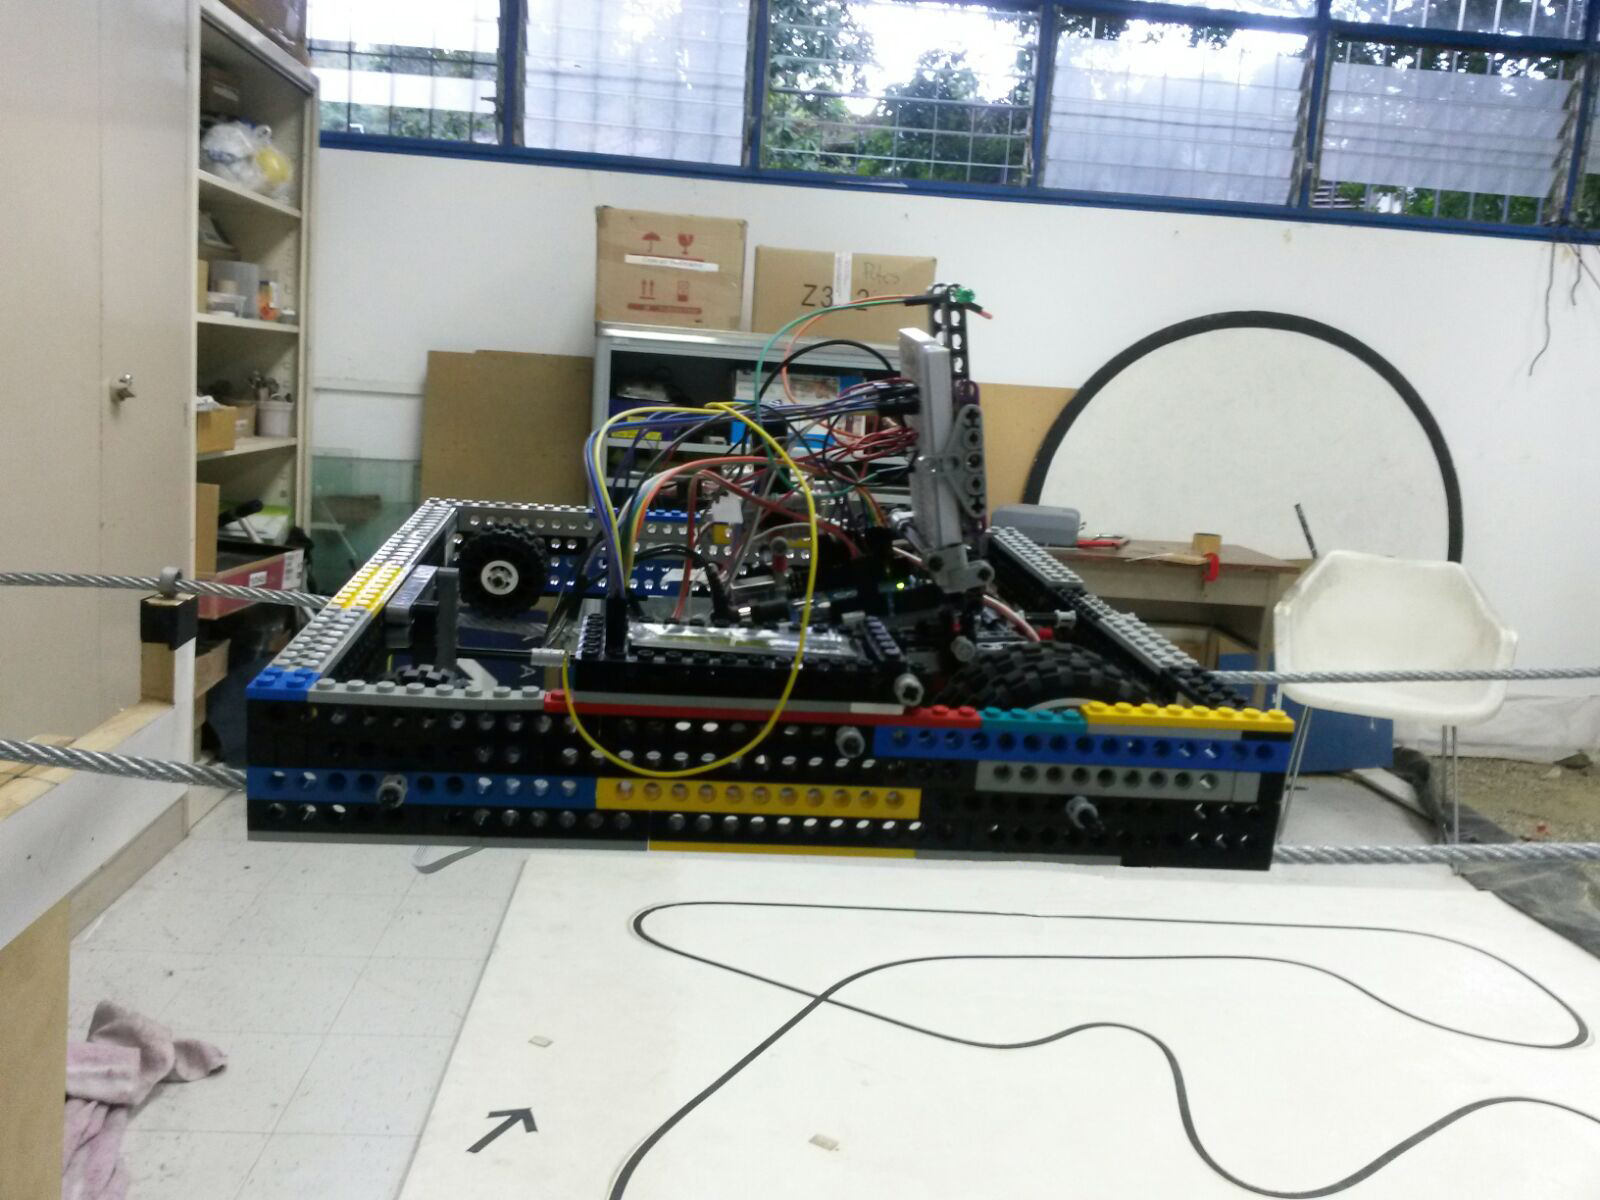
\includegraphics[scale=0.15,type=png,ext=.jpg,read=.jpg]{robot}
	\caption{Robot}
	\label{fig:robot}
\end{figure}

En esta superficie se encuentran el protoboard, la tarjeta y el resto de los componentes necesarios para realizar las tareas. \\

La tarjeta se encuentra sujeta a este diseño en la parte superior para facilitar la conexión de los componentes electrónicos.\\

Con el fin de conocer la distancia desde el punto de partida, tarea exigida en esta categoría, se toma como referencia las rotaciones que da el motor. 



\bigskip
\subsubsection{Diseño de la Sierra}

\bigskip

La sierra es la estructura encargada de cortar la maleza que se encuentra en las guayas que simulan los cables de electricidad. Es un motor DC que tiene indexado un disco de corte de esmeril que posee una lija de frente y desgasta el papel hasta removerlo de la línea. El motor se encuentra incorporado al robot con una caja de un solo ambiente hecha con piezas de LEGO\textregistered \vspace{2mm}. El disco se encuentra a un lado de la guaya, cerca de la misma para poder desgastar el papel de seda. La sierra se encuentra acoplado al lado derecho de la plataforma de tracción. \\

La versión actual de este componente presenta ciertos problemas que serán expuestos en la sección 3 de problemas encontrados.


\begin{figure}[htp]
	\centering
	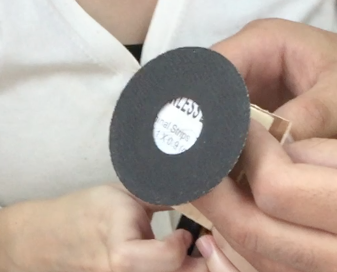
\includegraphics[scale=0.5,type=png,ext=.png,read=.png]{sierra}
	\caption{Sierra del Robot}
	\label{fig:sierra}
\end{figure}


\bigskip
\subsubsection{Diseño del Localizador de Puntos Calientes}

\bigskip

Es la estructura encargada de reconocer los puntos calientes. Consiste en una pequeña caja construida con LEGO\textregistered \vspace{2mm} donde se encuentra el sensor de reflectancia QTR-1RC, el cual detecta según un rango de números si lo que se encuentra observando es la guaya (color gris) o un punto caliente (color blanco).\\ 

 
El QTR-1RC se encuentra acoplado al frente del robot con la finalidad de, a parte de detectar los puntos calientes, distinguir los aislantes de forma que el robot pueda superar el obstáculo.\\


Para indicar la distancia desde la marca de salida se utilizará un display incorporado al robot. \\

\bigskip
\subsubsection{Diseño del Localizador de la Maleza en el corredor de servidumbre}

\bigskip

Es la estructura encargada de reconocer la maleza peligrosa bajo las líneas de transmisión. Consiste simplemente en un sensor de ultrasonido incorporado a la estructura móvil del robot.\\

Para mostrar la magnitud de la distancia correspondiente desde la marca de salida se utilizará el display incorporado al robot. \\



\bigskip

\subsection{Aspectos Electrónicos}
\bigskip


Entre los aspectos electrónicos destacan los siguientes:\\
 
\begin{itemize}
	\item Para reducir la cantidad de pines usados por el display se utilizó el BUS I2C.\\
	
	\item Debido al uso de un motor cuya fuente de alimentación no se encuentra regulada por el Arduino, se usó un regulador de voltaje LM7812 para estabilizar la salida de corriente.\\
	
	\item Los condensadores necesarios para el uso de ese regulador fueron de 1 $\mu$F y 0.33 $\mu$F.\\
	
	\item Al momento de detectar un punto caliente se enciende un LED rojo. Para indicar la maleza peligrosa se encenderá un LED verde. Un LED azul indicará si el robot se encuentra prendido o apagado. Cada LED lleva una resistencia de 220 $\Omega$.\\
	
	\item El robot se alimenta con 16 pilas AA.

\end{itemize}




\bigskip

\subsection{Aspectos Algorítmicos}
\bigskip

En el presente punto se desarrollarán los diversos aspectos algorítmicos del código implementado:\\ 

\begin{itemize}
	
	
	\item Debido al uso del BUS se utilizó la librería WIRE.h para poder habilitar LiquidCrystal{\_}I2C.h\\
	\item Para usar los servos, se utilizó la librería especial Servo.h.\\
	\item Una serie de condicionales fueron utilizados para aprovechar las ventajas de los sensores y resolver los problemas planteados.\\
	
\end{itemize}





\bigskip
\section{Problemas Encontrados}
\bigskip

A continuación se presentan los principales problemas encontrados
a lo largo del desarrollo del robot, en conjunto con posibles
soluciones.

\bigskip
\subsection{Problemas Estructurales}

\bigskip
Un gran problema en el diseño espacial del robot vino dado por
las limitaciones de espacio (un cubo de 30 cm$ ^{3} $). Si bien una de las ventajas de utilizar LEGO\textregistered \vspace{2mm} en la estructura del robot es que permite acoplar fácilmente las estructuras modulares. No obstante, debido a que estas piezas vienen con tamaños preestablecidos, dificulta alcanzar la precisión deseada. Esto podría resolverse con la ayuda de materiales que puedan modificarse a conveniencia.\\

Debido al peso del robot se hace difícil llegar hasta el punto más alto de la guaya.\\


\bigskip
\subsection{Problemas con la Sierra}
\bigskip

Uno de los problemas actuales de la sierra es su motor. Su peso y tamaño resulta inconveniente para el desarrollo del proyecto.\\

Se probó el uso de motores más pequeños pero la mayoría poseía no poseía suficiente torque para garantizar el avance continuo de la sierra. Los diferentes motores utilizados se muestran en la Figura \ref{fig:motor}.\\



\begin{figure}[htp]
	\centering
	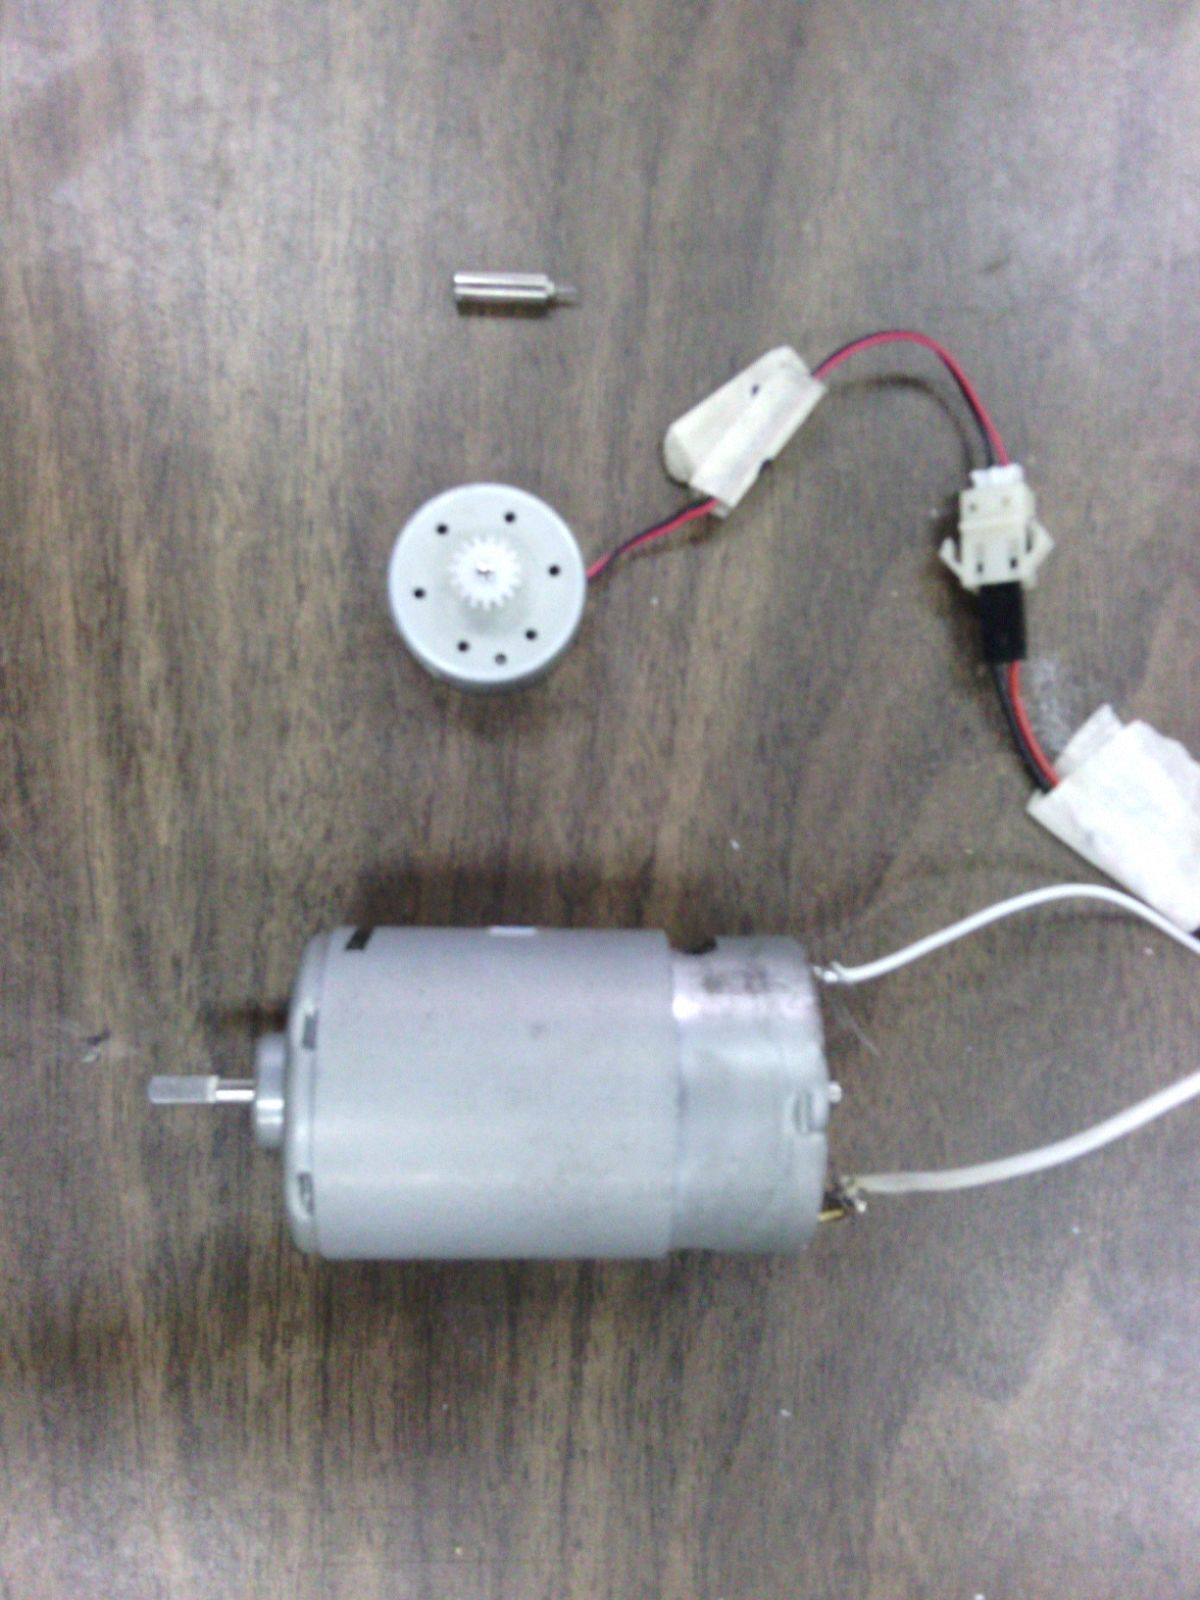
\includegraphics[scale=0.15,type=jpg,ext=.jpg,read=.jpg]{motor}
	\caption{Motores utilizados para la Sierra}
	\label{fig:motor}
\end{figure}

Por otra parte la sierra tarda un tiempo considerable en desgastar el papel de seda lo que resulta un problema significativo.\\ 

\bigskip
\subsection{Problema con el sensor de reflectancia QTR-1RC}
\bigskip

El mayor problema que se encontró con el sensor de reflectancia QTR-1RC fue que al pasar los aislantes el robot levanta gran parte de su estructura incluyendo el sensor. Esto hace que las lecturas hechas varíen en gran medida.  

\bigskip
\section{Conclusión}
\bigskip

El primer prototipo desarrollado probó ser una buena base para las siguientes etapas de desarrollo. Debido al diseño modular, los problemas que se enfrentan actualmente pueden ser atacados sin realizar fuertes cambios estructurales en el robot.\\

En la siguiente etapa, la prioridad será mejorar la subida del robot en la guaya ya que se le hace difícil llegar hasta el punto más alto de la línea de transmisión.\\

Por otra parte la sierra tarda de manera considerable en cortar el papel de seda lo que resulta un problema significativo.\\ 

Es posible que la limitación en el tamaño del robot sea una causa importante de las dificultades que se puedan presentar posteriormente.\\

Mediante el desarrollo del prototipo, se entendieron las ventajas y desventajas de variados tipos de construcción en LEGO\textregistered \vspace{2mm}, procedimientos de calibración, técnicas de detección de errores. Este conocimiento será de utilidad en la segunda etapa de desarrollo del robot.\\

\bigskip

\section*{Agradecimientos}
\bigskip

 Estamos profundamente agradecidos con todas las personas que muy amablemente donaron e hicieron posible con ello la participación en esta competencia y a la ayuda incondicional de Arturo Toro, María Victoria Jorge y María Gabriela Guzmán durante todo el proceso de construcción del robot. Para finalizar queremos agradecer los profesores Carolina Chang, Ivette Carolina Martínez y Guillermo Villegas por su guía y apoyo en todo momento. 


\bigskip
\begin{thebibliography}{1}

\bigskip
\bibitem[1]{reglas} http://www.unet.edu.ve/evento/unetbots/reglamentos/UNETBotsDesafio.pdf
\bibitem[2]{QTR}
https://www.pololu.com/product/958
\bibitem[3]{reglasg} http://www.unet.edu.ve/evento/unetbots/reglamentos/ReglamentoGeneral.pdf
\bibitem[4]{servo}
https://www.arduino.cc/en/Reference/Servo




\end{thebibliography}

\end{document}
